\section{Introduction}~\label{intro}

Recent advances in robotic systems have significantly improved autonomy in perception, manipulation, and planning across domains such as agriculture and household environments. Despite these advances, robots still frequently fail in real-world environments due to perception errors~\cite{kaipa2016addressing}, action execution failures~\cite{kaelbling1998planning}, and dynamic environmental changes~\cite{kurniawati2016online}. Consequently, many robotic systems still rely on human operators to continuously monitor execution and intervene when failures occur~\cite{dragan2013legibility, goodrich2008human}. However, requiring humans to constantly observe robotic systems and manually determine whether the robot is making reliable decisions is impractical for long horizon human--robot collaboration. Continuous monitoring increases cognitive workload and fatigue~\cite{chen2014human}, particularly in real-world deployments where robots operate for extended periods of time. Instead of relying on humans to identify failures after they occur, robotic systems should be able to recognize uncertain situations on their own and proactively request assistance only when necessary~\cite{sadigh2017active, leusmann2023understanding}. This raises two important challenges for collaborative robotic systems, namely (i) determining \textit{when} uncertainty becomes significant enough to require human intervention and (ii) deciding \textit{what} information should be queried to effectively resolve the uncertainty.



% Recent advances in robotic systems have achieved a high degree of autonomy in perception, manipulation, and planning across various domains such as agriculture and household environments. However, robots still fail due to perception errors~\cite{kaipa2016addressing}, action execution failures~\cite{kaelbling1998planning}, or dynamic obstacles~\cite{kurniawati2016online}, which requires human supervision. Existing human--robot collaborative systems has explored different roles for human operators to monitor the system and prevent potential failures~\cite{dragan2013legibility, goodrich2008human}. Despite these efforts, requiring continuous human oversight increases cognitive workload~\cite{chen2014human}. To overcome this limitation, it is important for robots to recognize uncertain situations on their own and request assistance only when necessary~\cite{sadigh2017active, leusmann2023understanding}. However, determining (i) \textit{when} uncertainty arises and deciding (ii) \textit{what} information to query in order to resolve the uncertainty remain significant challenges for robotic systems.


To address these challenges, we formulate robotic decision making as a POMDP~\cite{kaelbling1998planning} and develop a framework that jointly models symbolic knowledge~\cite{davis1993knowledge} and uncertainty within a unified structure. We adopt a STRIPS-style symbolic representation~\cite{fikes1971strips}, where the knowledge base is defined as a set of explicit facts. In addition, the system maintains a belief distribution over possible world states, which represent alternative hypotheses about the environment. As observations are collected, the system updates the belief over these states accordingly. \cp{By measuring the entropy of the belief distribution, the system estimates uncertainty over possible worlds} and determines \textit{when} to query a human. The system also determines \textit{what} to ask by selecting questions that are expected to maximally reduce the remaining uncertainty between competing world states. Since the interaction only requires simple feedback about the environment state, the proposed framework reduces user cognitive burden without requiring users to make planning decisions.

% To address these challenges, we formulate robotic decision making as a POMDP~\cite{kaelbling1998planning} and develop a framework that jointly models symbolic knowledge~\cite{davis1993knowledge} and uncertainty within a unified structure. We adopt a STRIPS style symbolic representation~\cite{fikes1971strips}, where the knowledge base is defined as a set of explicit facts. In addition, the system maintains a belief distribution over possible future states, referred to as possible worlds, which represent alternative hypotheses about the environment. As observations are collected, the system evaluates these hypotheses and updates the belief accordingly. % By quantitatively measuring the uncertainty over possible worlds, the system determines when to query a human and selects informative questions to reduce ambiguity.
% \cp{By quantitatively measuring the uncertainty over possible worlds using the entropy of the belief distribution}, the system determines \textit{when} to query a human and selects \textit{what} questions to ask in order to reduce ambiguity. Since the user only provides simple judgments about the environment state rather than action-level decisions or plan modifications, the proposed framework reduces cognitive burden.



% \cp{To address this problem, a limited number of prior works~\cite{} propose frameworks for quantifying uncertainty in decision-making problems. However, to the best of our knowledge, few studies integrate uncertainty estimation into robotic decision-making systems. In this work, we propose a unified framework that formulates robotic decision making as a POMDP over symbolic knowledge representations. The robot maintains possible world states and estimates uncertainty using the entropy of the belief distribution over these states. The system then identifies the states that contribute most to the uncertainty and asks the user questions to reduce ambiguity. Since the user only provides simple judgments about the environment state rather than action-level decisions or plan modifications, the proposed framework reduces cognitive burden.}

\begin{figure}[t]
\captionsetup{skip=0pt}
    \centering
    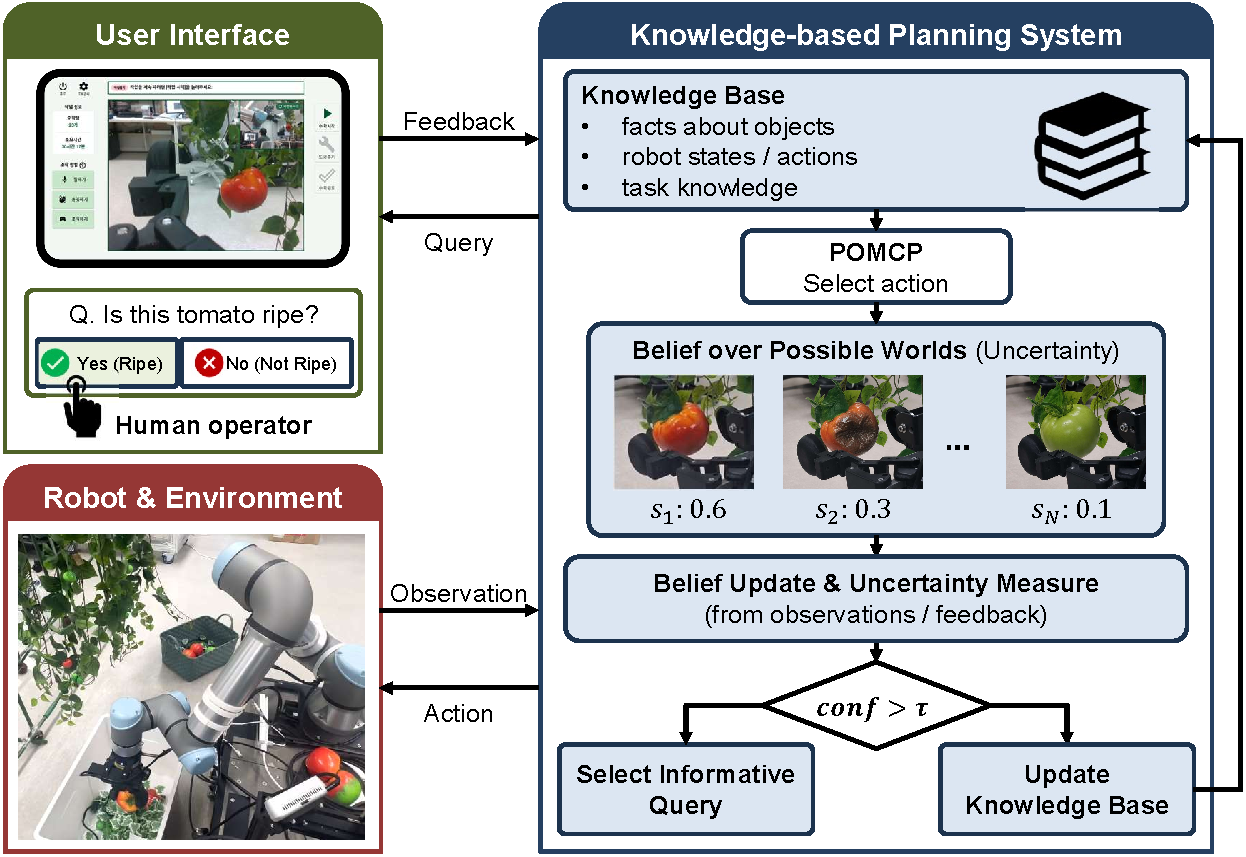
\includegraphics[width=0.7\linewidth]{figures/fig_overview.pdf}
    % 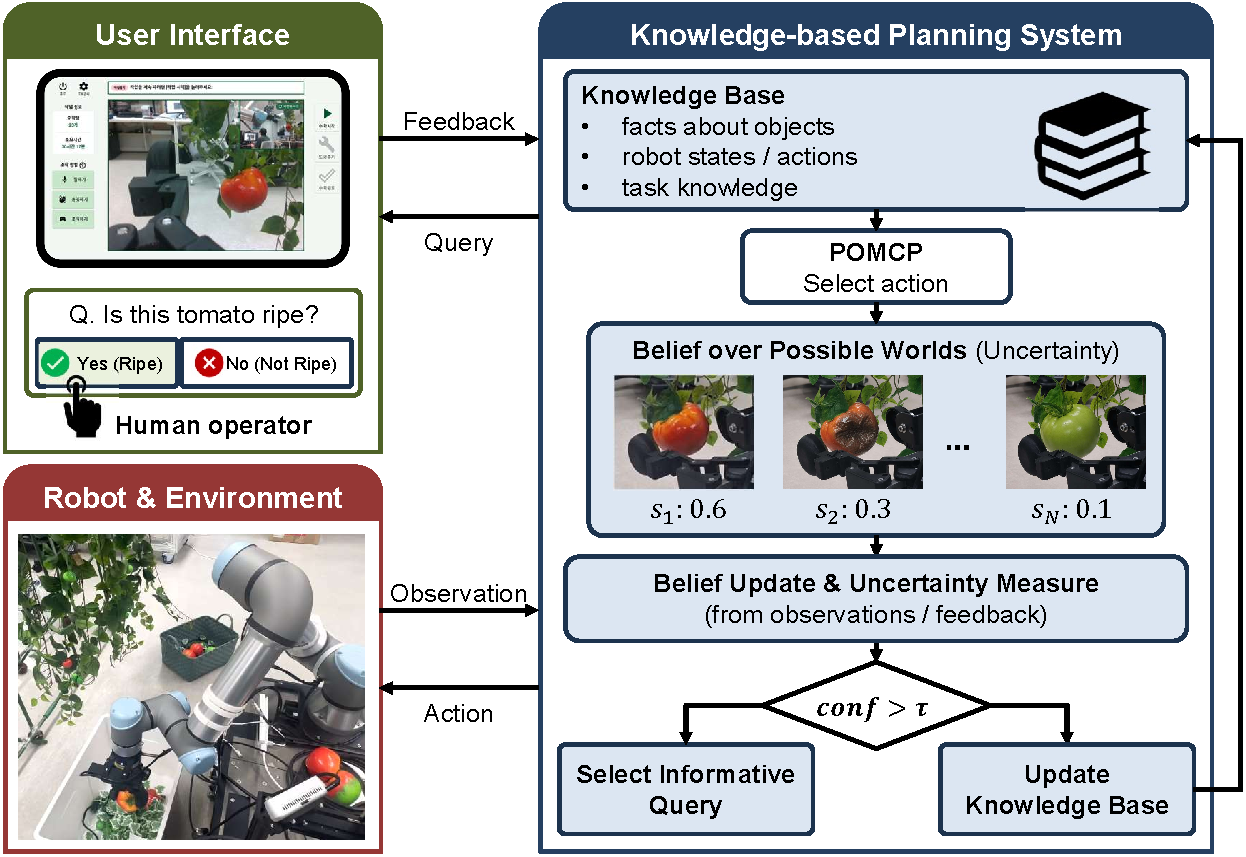
\includegraphics[width=0.98\linewidth]{figures/fig_overview.pdf}
    \caption{Overview of the proposed knowledge-based robotic system with uncertainty-aware planning. The system maintains a belief over possible worlds and updates it based on observations. If the uncertainty exceeds a threshold, the system selectively queries the user to resolve ambiguity. Otherwise, it continues autonomous planning and execution.}
    \label{fig:intro}
    % \vspace{-10pt}
\end{figure} 




% Building upon this framework, we design a comprehensive system architecture designed for robust robotic operation in real-world environments by implementing the framework, as shown in Fig.~\ref{fig:intro}. Anchored by a centralized knowledge base, the system integrates sensing, planning, feedback management, and user interface modules into a unified framework. Each module operates autonomously while asynchronously sharing and updating information through the knowledge base. This structure ensures that environmental data from sensors and direct user feedback are represented consistently and integrated immediately into the planning process.

\cp{We design a system architecture for real-world robotic operation based on this framework, as illustrated in Fig.~\ref{fig:intro}. The system performs decision making using a POMDP formulation, maintaining a belief over possible worlds and updating it based on observations. A centralized knowledge base integrates sensing, planning, feedback management, and user interface modules. Sensor observations and user feedback directly update the knowledge base and are shared across modules. This design maintains a consistent representation of information and ensures that planning uses the most up-to-date state.}


We evaluate the proposed approach in two domains, tomato harvesting and waste sorting. We demonstrate that our method reduces the number of interactions while maintaining or improving task success rates. In addition, user studies confirm that the proposed approach effectively reduces cognitive load during human–robot interaction.


% The main contributions are:
% \begin{itemize}
%     \item We present a robotic system that integrates knowledge-based reasoning with uncertainty-aware planning to enable effective human–robot collaboration.
%     \item We propose a unified pipeline that integrates uncertainty quantification with POMDP planning, enabling the system to proactively determine when to seek feedback and what to query.
%     \item We introduce an entropy-based method for refining queries, which reduces the interaction overhead.
%     \item We show through user studies that the proposed method reduces the workload on users.
% \end{itemize}


The main contributions of this work are as follows:
\begin{itemize}
    \item We propose a knowledge-based POMDP framework that explicitly represents uncertainty over symbolic world states for robotic decision making under partial observability.
    
    \item We introduce an entropy-based uncertainty estimation method that enables the robot to determine when human feedback is required during execution.
    
    \item We propose a query selection method that identifies informative environment states to determine what to ask in order to reduce uncertainty with minimal user interaction.
    
    \item We validate the proposed framework through user studies and show that it reduces user workload during human--robot collaboration.
\end{itemize}

